\documentclass[a4paper,12pt]{article}
\usepackage{graphicx}
\usepackage{caption}
\usepackage{subcaption}
\usepackage{float}
\usepackage[margin=1in]{geometry}
\usepackage{lmodern}
\usepackage{amsmath}
\usepackage{listings}

\begin{document}

\title{Relatório ELM}
\author{Eduardo}
\date{\today}
\maketitle

\section{Introduction}
Extreme Learning Machines (ELMs) are single-hidden layer feedforward neural networks where input weights are randomly initialized, and output weights are analytically determined. This report explores the impact of regularization on ELM's decision boundaries using synthetic datasets.

\section{Methodology}
The ELM classifier implemented includes:
\begin{itemize}
  \item Random initialization of input weights and biases with Glorot scaling.
  \item Activation functions: Sigmoid, ReLU, Tanh, and RBF.
  \item Regularized least squares for output weights: \( \mathbf{\beta} = (\mathbf{H}^T\mathbf{H} + \lambda \mathbf{I})^{-1}\mathbf{H}^T\mathbf{Y} \), where \( \lambda \) is the regularization parameter.
\end{itemize}

Two experiments were conducted:
\begin{enumerate}
  \item A synthetic 2D dataset using \texttt{make\_classification} with an 80-20 train-test split.
  \item The moons dataset with varying regularization parameters to visualize decision boundaries.
\end{enumerate}

\section{Results}
\subsection{Synthetic Dataset}
The ELM achieved a test accuracy of \textbf{94.00\%} on the synthetic dataset, demonstrating effective separation of classes.

\subsection{Decision Boundaries with Regularization}
Figure \ref{fig:dec_surf} shows decision boundaries for the moons dataset under different regularization strengths:
\begin{figure}[ht]
  \centering
  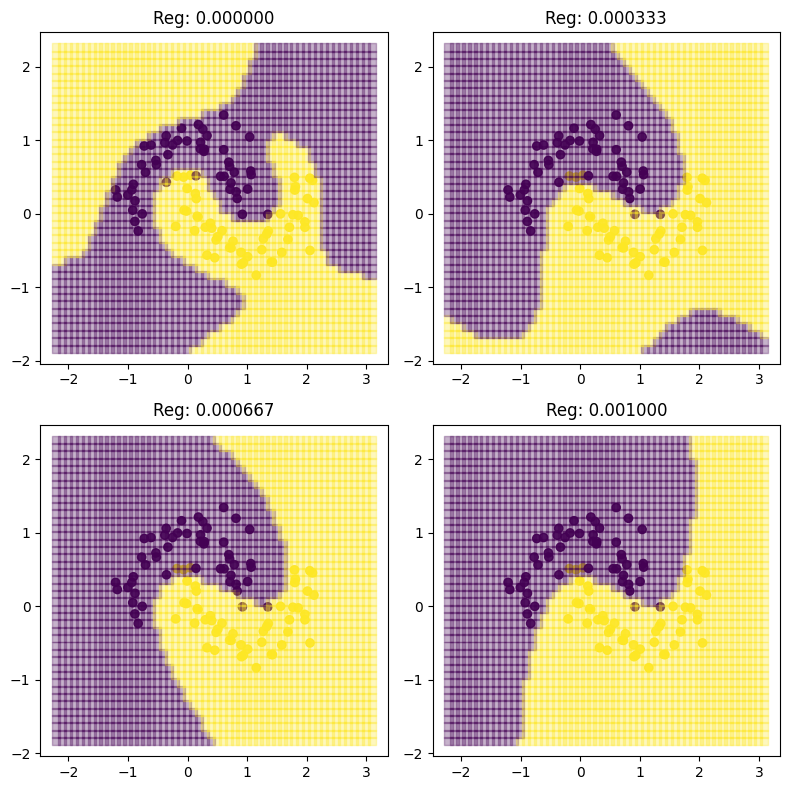
\includegraphics[width=0.9\textwidth]{dec_surf.png}
  \caption{Decision boundaries with varying regularization (\( \lambda \)). Top-left to bottom-right: \( \lambda = 0, 0.000333, 0.000667, 0.001 \). Higher \( \lambda \) smooths boundaries, reducing overfitting.}
  \label{fig:dec_surf}
\end{figure}

Key observations:
\begin{itemize}
  \item \( \lambda = 0 \): Complex boundary, potential overfitting.
  \item \( \lambda = 0.001 \): Smoother boundary, improved generalization.
\end{itemize}

\section{Conclusion}
Regularization in ELM controls model complexity by penalizing large weights. Higher \( \lambda \) values yield smoother decision boundaries, trading training accuracy for better generalization. The experiments validate the importance of tuning \( \lambda \) to balance bias and variance.

\end{document}